\documentclass[12pt]{article}

% ----------------------------------------------------------------------
% Define external packages, language, margins, fonts, new commands 
% and colors
% ----------------------------------------------------------------------
\usepackage[utf8]{inputenc} % Codification
\usepackage[english]{babel} % Writing idiom

\usepackage{listings}
\usepackage[dvipsnames]{xcolor}
\usepackage[most]{tcolorbox}
\usepackage{float}


\definecolor{codebg}{RGB}{245,245,245}
\definecolor{codeframe}{RGB}{200,200,200}

\lstdefinestyle{CiscoStyle}{
    backgroundcolor=\color{codebg},
    basicstyle=\ttfamily\small,
    keywordstyle=\color{blue},
    commentstyle=\color{gray},
    breaklines=true,
    showstringspaces=false,
    columns=fullflexible
}

\newtcblisting{configbox}{
    listing only,
    colback=codebg,
    colframe=codeframe,
    arc=3mm,
    boxrule=0.5pt,
    left=2mm,
    right=2mm,
    top=1mm,
    bottom=1mm,
    listing options={style=CiscoStyle}
}

\newtcblisting{largeconfigbox}{
    listing only,
    breakable,
    colback=codebg,
    colframe=codeframe,
    arc=3mm,
    boxrule=0.5pt,
    listing options={
        style=CiscoStyle,
        basicstyle=\ttfamily\scriptsize
    }
}

\usepackage{graphicx}
\usepackage[export]{adjustbox} % Align images
\usepackage{amsmath} % Extra commands for math mode
\usepackage{amssymb} % Mathematical symbols
\usepackage{anysize} % Personalize margins
    \marginsize{2cm}{2cm}{2cm}{2cm} % {left}{right}{above}{below}
\usepackage{appendix} % Appendices
\usepackage{cancel} % Expression cancellation
\usepackage{caption} % Captions
    \captionsetup{labelfont={bf}}
\usepackage{cite} % Citations, like [1 - 3]
\usepackage{color} % Text coloring
\usepackage{fancyhdr} % Head note and footnote
    \pagestyle{fancy}
    \fancyhf{}
    \fancyhead[L]{\footnotesize IST} % Left of Head note
    \fancyhead[R]{\footnotesize ULisboa} % Right of Head note
    \fancyfoot[L]{\footnotesize DDRS} % Left of Footnote
    \fancyfoot[C]{\thepage} % Center of Footnote
    \fancyfoot[R]{\footnotesize METI} % Right of Footnote
    \renewcommand{\footrulewidth}{0.4pt} % Footnote rule
\usepackage{float} % Utilization of [H] in figures
\usepackage{graphicx} % Figures in LaTeX
\usepackage[colorlinks = true, plainpages = true, linkcolor = istblue, urlcolor = istblue, citecolor = istblue, anchorcolor = istblue]{hyperref}
\usepackage{indentfirst} % First paragraph
\usepackage[super]{nth} % Superscripts
\usepackage{siunitx} % SI units
\usepackage{subcaption} % Subfigures
\usepackage{titlesec} % Font
    \titleformat{\section}{\Large\bfseries}{\thesection}{1em}{}
    \titleformat{\subsection}{\large\bfseries}{\thesubsection}{1em}{}
    \titleformat{\subsubsection}{\normalsize\bfseries}{\thesubsubsection}{1em}{}
    \fancyfoot[C]{\thepage}

% New and re-newcommands
\newcommand{\sen}{\operatorname{\sen}} % Sine function definition
\newcommand{\HRule}{\rule{\linewidth}{0.5mm}} % Specific rule definition
\renewcommand{\appendixpagename}{\LARGE Appendices}

% Colors
\definecolor{istblue}{RGB}{3, 171, 230}
\definecolor{dkgreen}{rgb}{0,0.6,0}
\definecolor{gray}{rgb}{0.5,0.5,0.5}

%%%%%%%%%%%%%%%%%%%%%%%%%%%%%%%%%%%%%%%%%%%%%%%%%%%%%%%%%%%%%%%%%%%%%%%%
%                                 Document                             %
%%%%%%%%%%%%%%%%%%%%%%%%%%%%%%%%%%%%%%%%%%%%%%%%%%%%%%%%%%%%%%%%%%%%%%%%

\begin{document}

% ----------------------------------------------------------------------
% Cover
% ----------------------------------------------------------------------
\begin{center}
    \begin{figure}
        \vspace{-1.0cm}
        
\includegraphics[scale = 0.1, left]{../../module 1/images/IST_A.png} % IST logo
    \end{figure}
    \mbox{}\\[2.0cm]
    \textsc{\Huge Performance Evaluation and Dimensioning of Networks and Systems}\\[2.5cm]
    \textsc{\LARGE METI}\\[2.0cm]
    \HRule\\[0.4cm]
    {\large \bf {Lab 2 Report} [\texttt{EN}]}\\[0.2cm]
    \HRule\\[1.5cm]
\end{center}

\begin{flushleft}
    \textbf{Authors:}
\end{flushleft}

\begin{center}
    \begin{minipage}{0.5\textwidth}
        \begin{flushleft}
            Jos\'e Oliveira (103771) \\
            Afonso Mendes (116024) \\
            Tiago Videira (116069)
        \end{flushleft}
    \end{minipage}%
    \begin{minipage}{0.5\textwidth}
        \begin{flushright}
            \href{mailto:jose.novais.oliveira@tecnico.ulisboa.pt}{\texttt{jose.novais.oliveira@tecnico.ulisboa.pt}}\\
            \href{mailto:afonsofmendes@tecnico.ulisboa.pt}{\texttt{afonsofmendes@tecnico.ulisboa.pt}}\\
            \href{mailto:tiago.g.videira@tecnico.ulisboa.pt}{\texttt{tiago.g.videira@tecnico.ulisboa.pt}}\\
        \end{flushright}
    \end{minipage}
\end{center}

\vspace{1.2cm}
\begin{center}
    \large \bf 2026/2027 -- \nth{1} Semester
\end{center}
 
\thispagestyle{empty}
\setcounter{page}{0}
\newpage

% ----------------------------------------------------------------------
% Contents
% ----------------------------------------------------------------------
\tableofcontents 
\newpage

% ----------------------------------------------------------------------
% Body
% ----------------------------------------------------------------------

% ======================================================================
\section{Introduction}

This report presents the solutions to the three exercises assigned to class~5 in Laboratory~2 of the Performance Evaluation and Dimensioning of Networks and Systems (DDRS) course. It follows the objective--approach--results--conclusion structure used in the Laboratory~1 report. The R scripts and generated figures are in the \texttt{scripts} directory; the supplied ALOHA theory function and attack trace are reused from \texttt{scripts\_helper}.

\newpage

\section{A. Discrete-time Markov chains}

\subsection{Bernoulli and 2-DTMC sample paths}

\textbf{Objective:} Compare Bernoulli processes with two-state discrete-time Markov chains (2-DTMCs) using two parameter pairs that have the same stationary mean but markedly different temporal behavior.

\textbf{Approach:} For a 2-DTMC with transition matrix
\[
P =
\begin{bmatrix}
\alpha & 1-\alpha \\
\beta & 1-\beta
\end{bmatrix},
\]
the stationary probability of state~1 is
\[
\pi_1 = \frac{1-\alpha}{1-\alpha+\beta}.
\]
The script \texttt{E1\_DTMCBernoulli.R} compares 200-step sample paths for $(\alpha,\beta)=(0.9,0.1)$ and $(0.1,0.9)$. Both have $\pi_1=0.5$, so each is paired with an independent Bernoulli process with success probability $0.5$. A fixed random seed makes the output reproducible.

\begin{figure}[H]
    \centering
    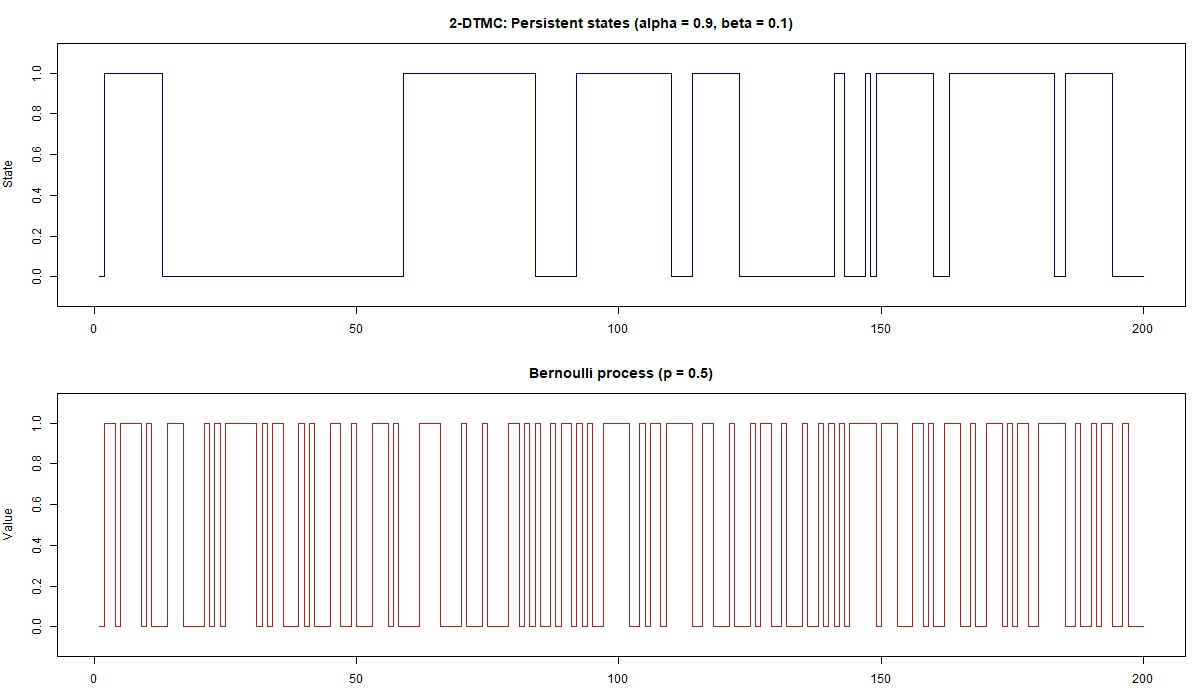
\includegraphics[width=0.9\textwidth]{../scripts/E1_DTMCBernoulli_alpha_0.9_beta_0.1.jpeg}
    \caption{Persistent 2-DTMC states compared with a Bernoulli process of the same mean.}
    \label{fig:class5-persistent}
\end{figure}

\begin{figure}[H]
    \centering
    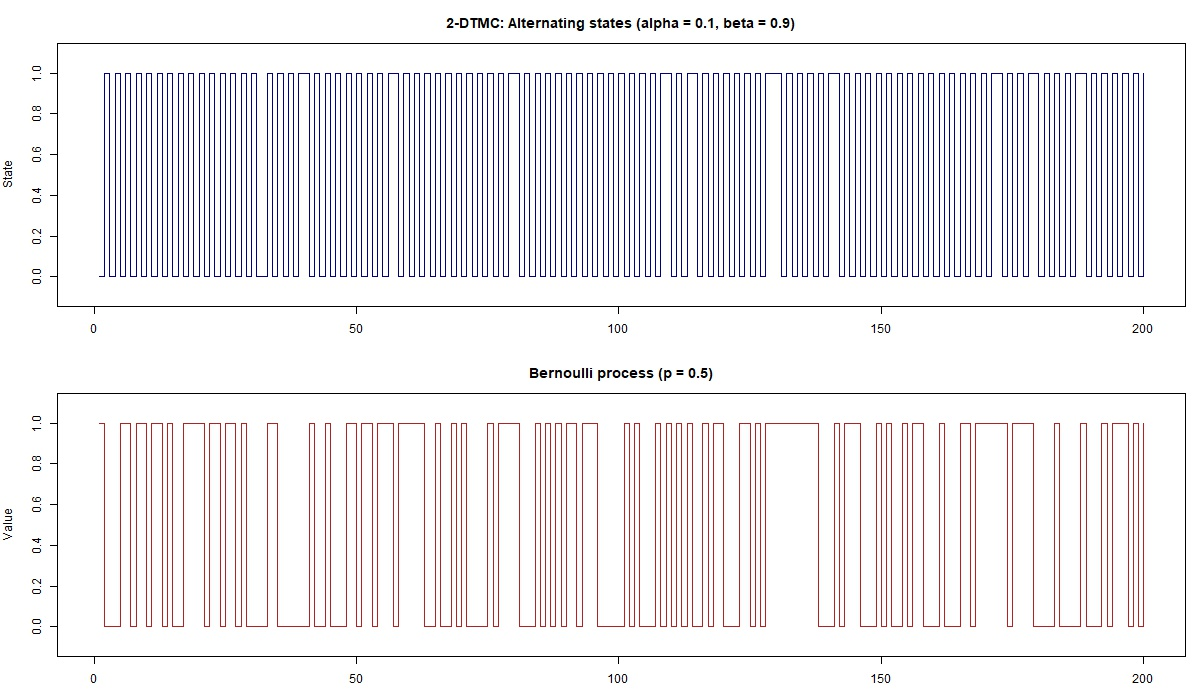
\includegraphics[width=0.9\textwidth]{../scripts/E1_DTMCBernoulli_alpha_0.1_beta_0.9.jpeg}
    \caption{Alternating 2-DTMC states compared with a Bernoulli process of the same mean.}
    \label{fig:class5-alternating}
\end{figure}

\textbf{Results and conclusion:} With $(0.9,0.1)$, a state is likely to persist, so the 2-DTMC exhibits long runs of zeros or ones. With $(0.1,0.9)$, transitions between the states are likely, producing an alternating pattern. In both cases the long-run fraction of ones is $0.5$, matching the Bernoulli mean, but the Bernoulli samples have no temporal dependence. A 2-DTMC can therefore model persistence, clustering, and alternation in a sequence; an independent Bernoulli process cannot represent these dependencies.

\subsection{Estimating transitions from the attack trace}

\textbf{Objective:} Estimate the transition probabilities of a 2-DTMC from the sequence of daily server attack indicators in \texttt{2dtmcdata.txt}.

\textbf{Approach:} The script \texttt{E2\_AttackDTMC.R} imports the supplied file with the tab separator specified in the exercise. It counts each consecutive transition $i\to j$ and divides by the number of transitions originating in state~$i$. The trace contains 2,000 observations and thus 1,999 transitions.

\begin{table}[H]
    \centering
    \caption{Estimated transition counts and probabilities for the attack trace.}
    \label{tab:attack-transitions}
    \begin{tabular}{c|rr|rr}
        & \multicolumn{2}{c|}{Transition counts} & \multicolumn{2}{c}{Estimated probabilities} \\
        Current state & To 0 & To 1 & To 0 & To 1 \\
        \hline
        0 (not attacked) & 623 & 577 & 0.5192 & 0.4808 \\
        1 (attacked) & 577 & 222 & 0.7222 & 0.2778 \\
    \end{tabular}
\end{table}

\textbf{Results and conclusion:} The estimated transition matrix, with rows denoting the current state, is
\[
\widehat{P} =
\begin{bmatrix}
0.5192 & 0.4808 \\
0.7222 & 0.2778
\end{bmatrix}.
\]
The fitted chain estimates an attack probability of approximately $0.3997$ in steady state. An attack is followed by another attack with estimated probability $0.2778$; otherwise, the process returns to the non-attacked state with probability $0.7222$. These are empirical estimates from this finite trace, rather than known properties of all server attacks.

\subsection{Slotted ALOHA}

\textbf{Objective:} Study the theoretical and simulated throughput of slotted ALOHA with a finite number of users, explain the effect of the parameters $N$, $\sigma$, and $p$, and compare ALOHA with carrier-sensing protocols.

\subsubsection{Theoretical throughput}

\textbf{Approach:} A system state is the number of backlogged users. A thinking user transmits with probability $\sigma$ in a slot, while a backlogged user transmits with probability $p$. Throughput is the long-run number of successful transmissions per slot. The script \texttt{E3\_SlottedALOHA.R} calls the supplied \texttt{aloha\_theo()} function to evaluate the stationary throughput over the requested parameter ranges.

\begin{figure}[H]
    \centering
    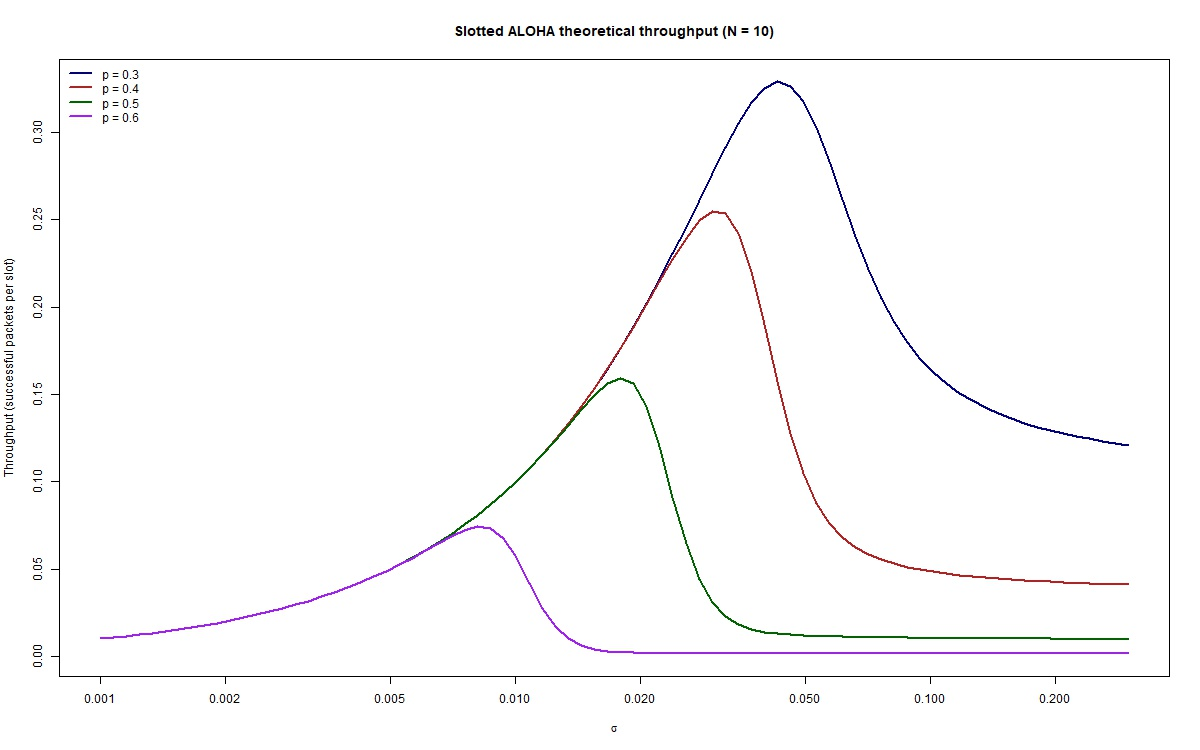
\includegraphics[width=0.85\textwidth]{../scripts/E3_ALOHA_N10.jpeg}
    \caption{Theoretical slotted-ALOHA throughput for $N=10$ and the four requested values of $p$.}
    \label{fig:aloha-n10}
\end{figure}

\begin{figure}[H]
    \centering
    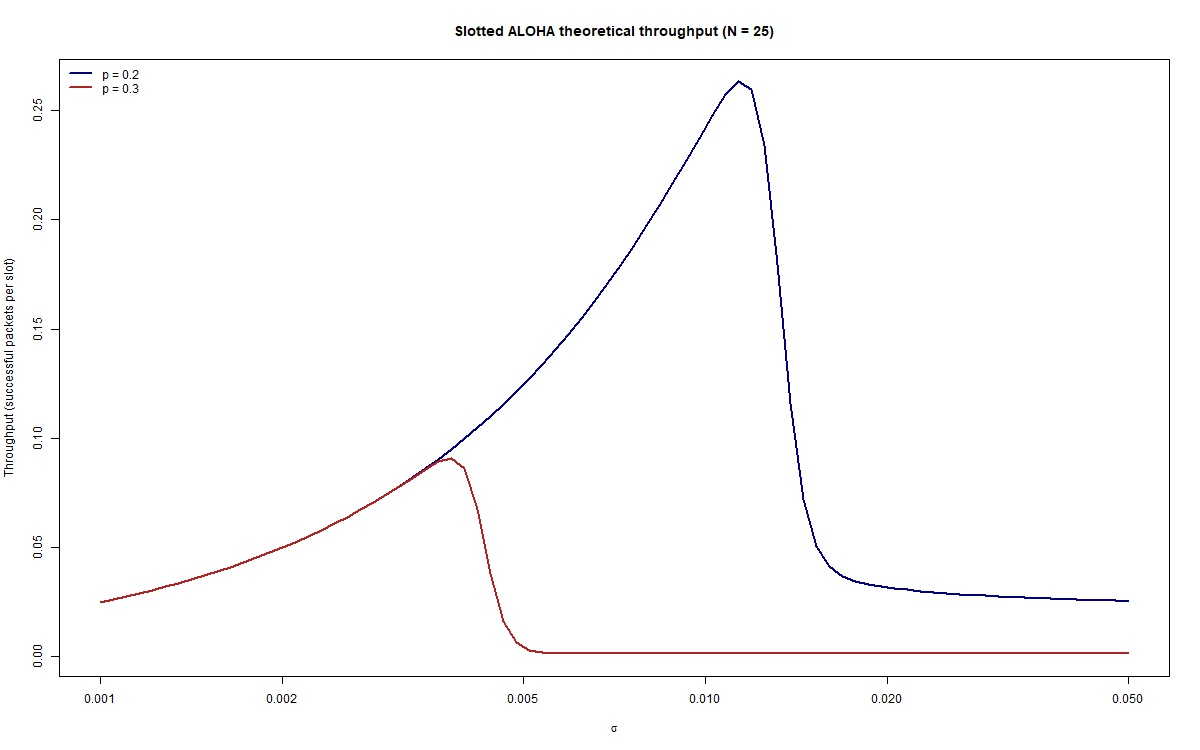
\includegraphics[width=0.85\textwidth]{../scripts/E3_ALOHA_N25.jpeg}
    \caption{Theoretical slotted-ALOHA throughput for $N=25$ and the two requested values of $p$.}
    \label{fig:aloha-n25}
\end{figure}

\textbf{Results and conclusion:} Increasing $\sigma$ causes more thinking users to attempt transmission. Initially this tends to increase throughput, but excessive attempts create collisions and move users into the backlog, so the throughput eventually peaks and can decrease. Increasing $p$ helps clear a backlog when few backlogged users are present, but when many are backlogged it also raises the chance of collisions. Increasing $N$ creates more potential traffic and contention; it does not guarantee higher throughput, since a larger population can spend more time in collision-heavy backlog states. The best operating point therefore depends jointly on all three parameters.

\subsubsection{Discrete-event simulation}

\textbf{Approach:} The same script runs one slot at a time. Each user attempts with the probability associated with its state. If exactly one user transmits, the slot is successful and a successful backlogged user returns to THINKING. If two or more transmit, there is a collision and each transmitting THINKING user becomes BACKLOGGED; existing backlogged users remain so. After a warm-up of 100,000 slots, throughput is estimated over 1,000,000 slots. The theoretical reference is computed by \texttt{aloha\_theo()}.

\begin{table}[H]
    \centering
    \caption{Theoretical and simulated throughput for three operating points.}
    \label{tab:aloha-comparison}
    \begin{tabular}{rrrrr}
        $N$ & $\sigma$ & $p$ & Theoretical & Simulation \\
        \hline
        10 & 0.001 & 0.3 & 0.01000 & 0.01004 \\
        10 & 0.100 & 0.3 & 0.16415 & 0.16309 \\
        10 & 0.100 & 0.6 & 0.00160 & 0.00157 \\
    \end{tabular}
\end{table}

\textbf{Results and conclusion:} The simulated estimates are close to their theoretical values for all three configurations. The results illustrate the sensitivity to the offered load and retransmission probability: the middle setting has the highest throughput, while raising $p$ to $0.6$ at the same $\sigma$ leaves more users contending in the backlog and substantially reduces successful transmissions.

\subsubsection{Comparison with CSMA and CSMA/CD}

ALOHA allows a user to transmit without first sensing whether the channel is occupied, so simultaneous attempts can collide. CSMA (Carrier Sense Multiple Access) reduces collisions by sensing the medium before transmitting. CSMA/CA, used by IEEE~802.11 wireless LANs, attempts to avoid collisions because a wireless station generally cannot reliably detect a collision while it is transmitting. CSMA/CD (Carrier Sense Multiple Access with Collision Detection) detects collisions during transmission and was used by shared, half-duplex Ethernet; modern switched full-duplex Ethernet does not use CSMA/CD. ALOHA-family random-access methods are also used in RFID tag anti-collision protocols and satellite/random-access links. Carrier sensing can improve channel efficiency when stations can sense one another, while ALOHA remains useful where sensing is unavailable or impractical.

\textbf{References:} GS1, \emph{EPC Radio-Frequency Identity Protocols Generation-2 UHF RFID}, for framed slotted-ALOHA tag inventory; IEEE~802.11 for wireless LAN medium access; and IEEE~802.3 for Ethernet, including the historical shared-medium collision-detection mechanism.

\section{Conclusion}

The three class~5 exercises demonstrate how DTMCs extend independent Bernoulli models by representing temporal dependence, how transition probabilities can be estimated directly from observed state changes, and how the stationary behavior of a contention protocol can be studied analytically and by simulation. The estimated and simulated results are consistent with the corresponding models, while also showing that finite data and operating parameters matter when interpreting performance.

\end{document}
